\autsection{The rosette sampler}{Fruzsina Bacso}

A suspended-particle rosette (SUPR) multi-sampler is a system which was developed for deep-ocean investigation. It enables detailed oceanographic research of hydrothermal plumes and abiotic and biotic plume processes. With this device, scientists are able to collect geochemical and microbial samples, which is very similar to what our goal is. Therefore we could use the SUPR sample collector design in the Europa-mission.
\cite{Breier20091579}

\subsubsection{The filtering head}
The multi-sampler is suited for filtering 24 discrete water samples and designed to host in situ optical sensors for immediate optical analysis.
The design allows multi-stage filtering which means that it is able to collect different particle size samples simultaneously and also this sequential filtering facilitates complementary chemical and microbial analysis. In addition it has a large diameter flow path so that only the filters are determining the flow rate.
The filtering head is built up from a housing and a filter rosette which is demonstrated in the following picture. 
\ref{fig:SUPR_head}

\begin{figure}[htb]
  \centering
  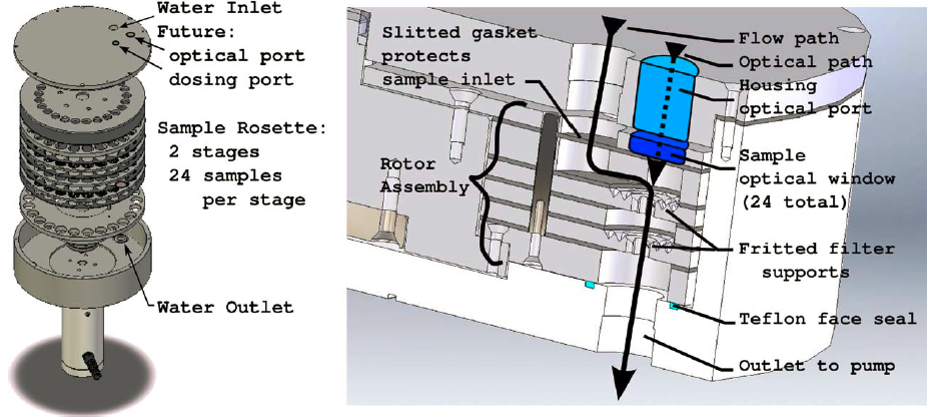
\includegraphics[scale=0.65]{figures/BFfig/SUPR_head}
  \caption{The suspended-particle rosette multi-sampler  }
  \label{fig:SUPR_head}
\end{figure}

The filtering rosette has several plates on top of each other which ensure and control the flow of the water. All 24 sample locations has an inlet, a closure, a lateral offset, a stack of two filter stages and an outlet. A rotor assembly controls the sample collection by rotating the filters one by one as it is filled and the water flow should be provided by a pump which is described in a different chapter.
The filter supporters can be seen on the picture below. 
\ref{fig:Filters}

\begin{figure}[htb]
  \centering
  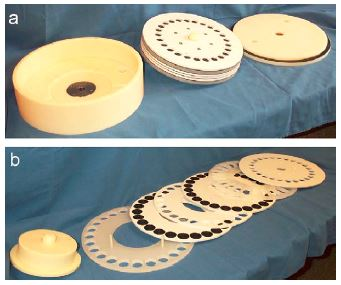
\includegraphics[scale=0.65]{figures/BFfig/Filters}
  \caption{The plates that support the filters}
  \label{fig:Filters}
\end{figure}

With this solution for the sampling we ensure a simple and brisk collection of the molecules. In addition the design could be capable of supporting the further analysis of the samples regarding all the instruments if each measuring equipment is rotated to the the optical window.
In the following table the SUPR sampler specifications can be seen.
\ref{fig:SUPR_spec}

\begin{figure}[htb]
  \centering
  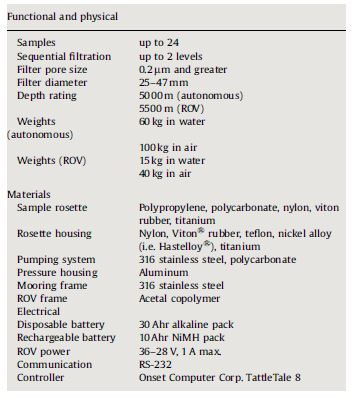
\includegraphics[scale=0.8]{figures/BFfig/SUPR_spec}
  \caption{The SUPR specifications}
  \label{fig:SUPR_spec}
\end{figure}